\documentclass{article}
\usepackage{graphicx} % Required for inserting images
\usepackage[a4paper, total={6in, 10in}]{geometry}
\usepackage{hyperref}
\usepackage{amsmath}
\usepackage{amssymb}
\usepackage{pgfplots}
\usepackage{tikz}
\usepackage{float}
\pgfplotsset{width=10cm,compat=1.9}
\usepgfplotslibrary{external}
\tikzexternalize

\title{Dayan and Abbott Notes}
\author{Rory Bedford}
\date{August 2024}

\begin{document}

\maketitle

These notes are written for the neuroscience reading group at the LMB, and are therefore aimed at biologists, with a less quantitative background. Some topics within Dayan and Abbott will be mathematically tricky for these readers, so my intention here is to give an overview of many of the topics covered to make things more digestible. Focus is therefore on understanding concepts broadly and how they relate to actual neurobiology, without getting too bogged down in derivations. That said, some familiarity with linear algebra, multivariate calculus and probability theory are still prerequisites for this. If you need a reference for these, I would highly recommend the first half of the textbook \href{https://mml-book.github.io/}{Mathematics for Machine Learning}. The appendix of Dayan and Abbott is also a fantastic resource.\\

The book is split into three main sections. In the first section, we look at how neurons encode information about the environment. In the second section, we look at biophysical models of neurons such as the Hodgkin-Huxley model, and work our way up to modelling biophysically plausible neural networks. In the final section, we look at learning, including mathematical models of plasticity, some basic reinforcement learning, and some Bayesian inference methods.\\

Note that my discussion for each chapter does not follow the material in the book in order but jumps around a little. I therefore reference the corresponding section in the book.

\section{Chapter 1 - Neural Encoding I}

In this chapter, we first look at neuron spike trains and firing rates, which are two different ways of thinking about a neuron's activity. We look at the relationship between these two forms, and how to convert between the two. We also have a first look at neural encoding, with neuron tuning curves and spike-triggered averages.

\subsection{Spike trains and firing rates}

Neurons fire action potentials at discrete points in time. If we measure a neuron's activity in a single trial, we end up with a list of times $t_i$ for $i = 1,2,...,n$ for n spikes, called a spike train. However, neurons don't work with infinite precision; there is some noise inherent in the timings of these action potentials. We therefore seek an alternate description of a neuron's activity that describes the \textit{rate} at which it is firing, not the exact times of its spikes. The spike-count rate is the neuron's firing rate measured across the entire trial. For a trial of length T:

\begin{equation*}
    r = \frac{n}{T}
\end{equation*}

The problem with this is that it doesn't account for variation of a neuron's firing rate within a trial, which is an important aspect of how neurons encode information. We therefore seek a firing rate \textit{function}, that varies with time, $r(t)$. This function is an abstraction that is a very useful way to think about neural activity given that spike trains are necessarily stochastic. We can think of it as being the same as the spike-count rate as above, but instead of considering the entire trial, we bin the trial into small windows of length $\Delta t$. We can then think of the function $r(t)$ as being the firing rate in the window $t$ to $t+\Delta t$, ie., the number of spikes in this window divided by $\Delta t$. This is not very useful if we are only considering one spike train, but if we perform the same recording across many trials, we can average their results to get a good description of a neuron's activity. Furthermore, the more trials we have, the smaller we can make the window $\Delta t$, and the more precise of firing rate function becomes.\\

\begin{figure}[ht]
\centering
    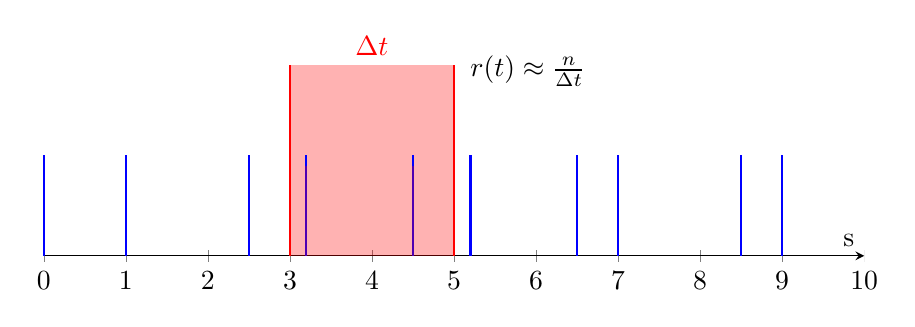
\begin{tikzpicture}
        \begin{axis}[
            width=12cm,
            height=4cm,
            axis y line=none,
            axis x line=middle,
            xmin=0, xmax=10,
            ymin=0, ymax=2,
            xlabel={s},
            clip=false
        ]
        
        % Spike train for a single neuron (small vertical lines)
        \addplot+[ycomb, thick, mark=|, mark size=2pt] 
            coordinates {
                (0, 1)
                (1, 1)
                (2.5, 1)
                (3.2, 1)
                (4.5, 1)
                (5.2, 1)
                (6.5, 1)
                (7, 1)
                (8.5, 1)
                (9, 1)
            };
        
        % Sliding window
        \fill[red, opacity=0.3] (axis cs:3,0) rectangle (axis cs:5,2);
        \draw[red, thick] (axis cs:3,0) -- (axis cs:3,2);
        \draw[red, thick] (axis cs:5,0) -- (axis cs:5,2);
        \node[red] at (axis cs:4,2.2) {$\Delta t$};

        \node[anchor=north] at (axis cs:5.9, 2.2) {$r(t) \approx \frac{n}{\Delta t}$};
        
        \end{axis}
    \end{tikzpicture}
\end{figure}

If we let the window size get infinitely small, then each window either catches a spike, or it doesn't. In this case, the firing rate is zero everywhere, apart from at the exact locations of a spike, at which it is infinite. The function that describes this is the dirac delta function $\delta (t)$. This function has the important property that it integrates to 1, and can therefore be used to 'pick out' values of a continuous function from inside an integral:

\begin{equation*}
    \int dt' \delta (t-t') f(t') = f(t)
\end{equation*}

We can now represent our spike train as a continuous function $\rho (t)$, rather than just a set of spike times, given by:

\begin{equation*}
    \rho (t) = \sum_{i=1}^n \delta(t-t_i)
\end{equation*}

For clarity, $\rho(t)$ is the particular function that we measure when recording a neuron's spiking activity. This is generated stochastically from the true underlying firing rate $r(t)$, which doesn't spike but gives a varying firing \textit{rate} over time.\\

We now need to look at how to convert between these two representations of a neuron's activity - ie, how to estimate $r(t)$ from a set of measured spike trains $\rho(t)$, and additionally, how to sample a spike train from a firing rate function.

\subsection{Spike train smoothing}

If we could record an infinite number of trials, then our simple window method above would converge to the true firing rate as the window size gets infinitely small. In practise, however, we generally need to estimate the firing rate from a finite number of trials. To do this, we smooth out our set of spike trains by performing a \textit{convolution} with a \textit{window} function $w(\tau)$. A convolution refers to the process of integrating our function of interest with a small sliding window function, sometimes called a kernel, as follows:\\

\begin{equation*}
    r(t) \approx \int_{- \infty}^{\infty} d\tau w(\tau) \rho(t-\tau)
\end{equation*}

If you think carefully about this equation, you see that at time t, we centre our window function at t, then compute the values of the window function at all neighbouring spikes, and add their values to give an estimate of the firing rate, as shown below. Also note that in practise, you can average this method over many trials where you have recorded the same neuron to get better results.\\

\begin{figure}[H]
    \centering
    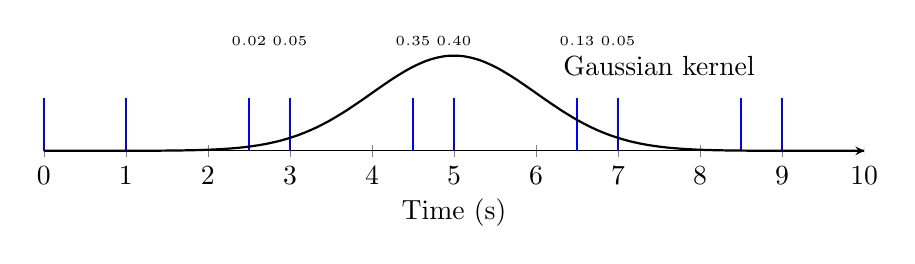
\begin{tikzpicture}
        \begin{axis}[
            width=12cm,
            height=4cm,
            xlabel={Time (s)},
            xlabel style={at={(axis description cs:0.5,-0.2)}, anchor=north},
            axis y line=none,
            axis x line=bottom,
            xmin=0, xmax=10,
            ymin=0, ymax=2,
            clip=false,
            domain=0:10
        ]
        
        % Spike train for a single neuron (small vertical lines)
        \addplot+[ycomb, thick, mark=|, mark size=2pt] 
            coordinates {
                (0, 0.5)
                (1, 0.5)
                (2.5, 0.5)
                (3, 0.5)
                (4.5, 0.5)
                (5, 0.5)
                (6.5, 0.5)
                (7, 0.5)
                (8.5, 0.5)
                (9, 0.5)
            };
        
        % Gaussian kernel
        \addplot[
            domain=0:10,
            samples=100,
            thick,
            black,
            samples=50,
            unbounded coords=jump,
            smooth
        ] {exp(-((x-5)^2)/(2*1^2))}; % Gaussian function with mean 5 and stddev 1

        \node[anchor=north] at (axis cs:7.5, 1.1) {Gaussian kernel};

        \node[anchor=south, font=\tiny] at (axis cs:2.5, 1) {$0.02$};
        \node[anchor=south, font=\tiny] at (axis cs:3, 1) {$0.05$};
        \node[anchor=south, font=\tiny] at (axis cs:4.5, 1) {$0.35$};
        \node[anchor=south, font=\tiny] at (axis cs:5, 1) {$0.40$};
        \node[anchor=south, font=\tiny] at (axis cs:6.5, 1) {$0.13$};
        \node[anchor=south, font=\tiny] at (axis cs:7, 1) {$0.05$};
        
        \end{axis}
    
    \end{tikzpicture}


    \begin{equation*}
        r(5) \approx 0.02 + 0.05 + 0.35 + 0.40 + 0.13 + 0.05\\
        \approx 1 \text{Hz}
    \end{equation*}
\end{figure}

Since our Gaussian window function varies smoothly, the effect is to smooth out the firing rate function. Smoothing the firing rate captures the fact that a spike train is generated stochastically from the firing rate - the smoother we make it, by widening the window width, the more we get a general rate, and the less the precise spike timings matter. The effects of using different window functions is shown in Figure 1.4 in the book.

\subsection{Poisson processes}

Having seen how we can estimate the firing rate from a set of recorded spike trains, we also want to consider how spike trains are actually generated from a given firing rate function.\\

First of all, note that we can easily calculate the mean number of spikes in a trial, as follows:

\begin{align*}
    \mathbb{E} [N] &= \int_0^T r(t)dt\\
    &= rT \text{ if r constant}
\end{align*}

However, this tells us nothing about the distribution of spikes around this mean rate. The most basic way to generate spikes is to use a Poisson process. Consider the probability of there being a spike in the window $t$ to $t+\Delta t$. As $\Delta t \to 0$, the probability of there being 2 or more spikes in this box falls to 0, so we only need to consider the possibility of there being 0 or 1 spikes in this box. This is just a coin flip, or Bernoulli trial, with the probability of there being a spike being given by $P(\text{spike})=r(t)\Delta t$. Computationally, you could simulate a spike train by splitting your trial into a finite set of small boxes of size $\Delta t$, and putting a spike in each box with this probability.\\

In the case of a homogeneous firing rate - that is, one that is constant for the whole trial, we can say a bit more about the distribution of the number of spikes in a trial. This is done by counting all the different ways we can get n spikes in a finite set of boxes in a trial using combinatorics, and adding their probabilities, then letting our box sizes tend to zero, while using something called Sterling's approximation to give the following nice result:

\begin{equation*}
    P[N=n] = \frac{(rT)^n}{n!} \exp(-rT)
\end{equation*}

Which is the Poisson distribution with mean $rT$.\\

An issue with this simplified model is that we assume the probabilities of a spike being in any bin is independent of the probability of a spike being in any other bin. This is obviously false, and the most major way this is violated is due to a neuron's refractory period - that is, if it spikes, the immediately following bins are extremely unlikely to also spike, regardless of how high the firing rate is. More complex models are able to incorporate a refractory period - in particular, the book discusses methods that sample interspike intervals to generate spike trains. For the homogeneous poisson process, the interspike interval follows an exponential distribution (the derivation in the book is quite straightforward), but this can be modified to a gamma distribution, which can make it almost impossible for a neuron to spike in the refractory period following a different spike.

\subsection{Tuning curves}

So far, we've only considered a neuron's activity in isolation. We now being our exploration of how a neuron can encode information about a stimulus. Chapter 1 really only makes a cursory first pass at this, but it gives a good flavour of what's to come.\\

First of all we consider the concept of a tuning curve. Tuning curves capture the relationship between the values of a stimulus and the mean firing rate of a neuron that encodes this stimulus. They are therefore a useful way of characterising the selectivity of a neuron to sensory information.\\

Here, we make the simplification that a neuron only encodes information via its mean firing rate - ie, there is no temporal encoding of information, only $<r>$ matters. We consider a parameterised stimulus $s$. For example, the book shows a moving bar in Figure 1.5(A) with its angle of rotation as the parameter of the stimulus. We then simply hold this parameter constant and record the neuron's activity, and calculate its mean firing rate over a trial of given duration. We can vary the value of the parameter(s) across different trials, to build up a picture of how the mean firing rate varies as the stimulus varies. We can then perform any type of curve fitting we want to this dataset to obtain a tuning curve.\\

This is a useful but slightly limited thing to do. It tells us nothing about how a neuron's activity varies around its mean firing rate. Some of this information could be very useful - for example, think of a neuron in an oscillatory system; information could certainly be encoded in the frequency of its response. A tuning curve would assign the same response to neurons with wildly different oscillating frequencies and would completely miss this encoding. It also can't account for temporal changes in parameters of the stimulus during a trial. Furthermore, many natural stimuli would be almost impossible to effectively parameterise - it therefore only really applies to simple stimuli such as gratings for vision.

\subsection{Spike-triggered average}

Another fundamental concept is the spike-triggered average. This is a way of characterising what type of stimulus is most likely to drive a spike. At present we will just define what a spike-triggered average actually is; justification for why this is useful comes in the next chapter when we study receptive fields, which essentially encompass these ideas and tuning curves.\\

At present, we once again have a parameterised stimulus, which we now allow to vary with with time, $s(t)$. We won't worry exactly how it varies - this will be considered in the next chapter. All we need to do to compute the spike-triggered average, is to record a neuron's activity alongside this varying stimulus in a trial. We then pick a window of finite time, and take the mean of the changing stimulus across all the windows preceding all spikes in the recording. We then average this result over any trials. This is described by the following equation:

\begin{equation*}
    C(\tau) = \langle\frac{1}{n}\sum_{i=1}^n s(t_i-\tau)\rangle
\end{equation*}

Equation (1.20) also covers the integral forms of this equation in terms of $\rho(t)$ and $r(t)$. It's actually really useful to look at these to check your understanding of our previous discussion on firing rates vs spike trains. Below also shows a visual representation of the spike-triggered average. All we do is take the stimulus in the windows preceding each spike, as shaded, and average them, to obtain $C(\tau)$.\\

\begin{figure}[H]
    \centering
    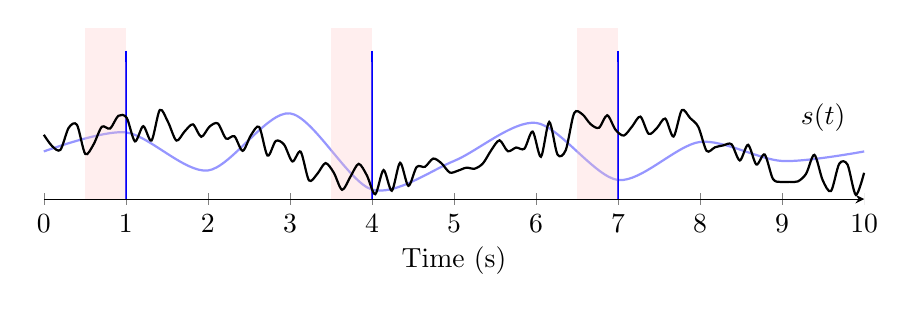
\begin{tikzpicture}
        % Define some colors for the stimulus and STA window
        \definecolor{stimuluscolor}{RGB}{150, 150, 255}
        \definecolor{stawindowcolor}{RGB}{255, 200, 200}
        
        \begin{axis}[
            width=12cm,
            height=4cm,
            xlabel={Time (s)},
            xlabel style={at={(axis description cs:0.5,-0.2)}, anchor=north},
            axis y line=none,
            axis x line=bottom,
            xmin=0, xmax=10,
            ymin=0, ymax=2,
            clip=false,
            domain=0:10
        ]

        % Randomly changing stimulus (using sine function as an example)
        \addplot [smooth, thick, stimuluscolor] 
            table[x=x, y=y] {
                x y
                0 0.5
                1 0.7
                2 0.3
                3 0.9
                4 0.1
                5 0.4
                6 0.8
                7 0.2
                8 0.6
                9 0.4
                10 0.5
            };

        % Spike train for a single neuron (small vertical lines)
        \addplot+[ycomb, thick, mark=|, mark size=2pt, color=blue] 
            coordinates {
                (1, 1.5)
                (4, 1.5)
                (7, 1.5)
            };

        % Shaded STA windows preceding each spike
        \foreach \x in {1, 4, 7} {
            \addplot [
                domain=\x-0.5:\x,
                samples=2,
                fill=stawindowcolor,
                fill opacity=0.3,
                draw=none
            ] {1.8} \closedcycle;
        }

        % Gaussian kernel
        \addplot[
            domain=0:10,
            samples=100,
            thick,
            black,
            smooth
        ] {0.5 + 0.3 * sin(2*pi*10*x) + 0.2 * rand};

        \node[anchor=north] at (axis cs:9.5, 1.1) {$s(t)$};

        \end{axis}
    \end{tikzpicture}

\end{figure}

\end{document}
